\section{The Dataset}\label{sec:dataset}
\subsection{Data Generation}


\subsection{Data Scaling and Transformations}
We shall briefly discuss how the training data is transformed before training.
The targets in the dataset of NLO cross sections can span several orders of magnitude. For practical training of BNNs, this would require
model parameters that also span several orders of magnitude. The result will usually be overflow and thus unsucessful training of the models.
Therefore, we have chosen to map the targets using the base-10 logarithm, i.e $y \mapsto \log_{10}(y)$. More generally, we could choose any base-$a$ logarithm. A practical consideration here is that once the model is trained, any prediction it produces must be transformed back using
the inverse mapping. As we increase the value of $a$, the precision the model can predict decreases. Thus a small error in log-space 
can result in a large error in what we may refer to as target space the larger the value of $a$ is. 


\section{Performance Metrics}\label{seq:perf_metrics}
In this section, we will discuss the performance metrics used to benchmark and measure the performance of the models trained in this thesis.
Due to the inherent probabilistic nature of the models trained, any output the model produces will be a distribution from which we can calculate
a sample mean and variance.

\subsection{Relative Error}
The first and simplest form of performance metric we can use is the \textit{relative error} which is defined as
\begin{equation}
    \epsilon(x^*) = \frac{y_\text{true}- \hat{y}_\text{mean}(x^*)}{y_\text{true}},
\end{equation}
where $y_\text{true}$ is the true target and $\hat{y}_\text{mean}(x^*)$ is the sample mean of the empirical predicitive distribution of the model.

\subsection{Standardized Residuals}
A particularly useful way to represent how well a probabilitic model performs is to study its \textit{standardized residual} which is given by
\begin{equation}
    z(x^*) = \frac{y_\text{true} - \hat{y}_\text{mean}(x^*)}{\hat{\sigma}(x^*)},
\end{equation}
where $\hat{\sigma}(x^*)$ is the square-root of the sample variance. The mathematical representation of the targets $y$ is that they can be decomposed as
\begin{equation}
    y = f(x) + \delta,
\end{equation}
for some true function $f(x)$ and a random noise $\delta \sim \mathcal{N}(0, 1)$, i.e it is distributed according to a standard Normal distribution. But in the case of data produced by \texttt{Prospino}, the noise is neglible which means that $y \approx f(x)$. The regression error obtained through the sample variance is therefore dominated by the predictive distribution computed by the model itself. A good model 



\section{Results}\label{sec:results}
\subsection{Benchmarks of Hyperparameters}\label{subsec:benchmarks}
\subsubsection{Baseline Model}
\subsubsection{Pretraining}
\subsubsection{Burn-in length}
\subsubsection{Number of model parameters}

\subsection{Neutralino-Neutralino Cross Sections}\label{subsec:neuralino_experiments}

\begin{table}[h!]
    \centering
\begin{tabular}{c@{\hspace{1cm}}c@{\hspace{1cm}}c@{\hspace{1cm}}c@{\hspace{1cm}}c@{\hspace{1cm}}c}
\hline
    Burn-in steps & \makecell{Number \\of \\steps between} & Kernel & \makecell{Number \\ of \\ results} & \makecell{Pretraining \\ epochs} & \makecell{Pretraining \\ batch size} \\
\hline
    2500 & 10 & NUTS & 1000 & 1000 & 32 \\
\hline
\end{tabular}
\caption{
    The table shows the training configuration used to sample the models listed in table~\ref{tab:deep_models}.
}
\label{tab:NN_mse_scores}
\end{table}


\begin{table}[h!]
    \centering
\begin{tabular}{c@{\hspace{1cm}}c@{\hspace{1cm}} c}
\hline
      Model number & Architechture & Number of parameters \\
\hline
    1 & 5-50-1 & 351\\
    2 & 5-50-50-1 & 2901\\
    3 & 5-50-50-50-1 & 5451\\
    4 & 5-50-50-50-50-1 & 8001\\
    5 & 5-50-50-50-50-50-1 & 10551\\
\hline
\end{tabular}
\caption{
    The table shows the models used in this section. For each model, 1000 sampled networks are used to
    generate each result shown in this section. The architecture describe number of nodes per layer.
    For each hidden layer, the same activation function is used. The final layer uses an identity function.
}
\label{tab:deep_models}
\end{table}

\begin{figure}
    \centering
    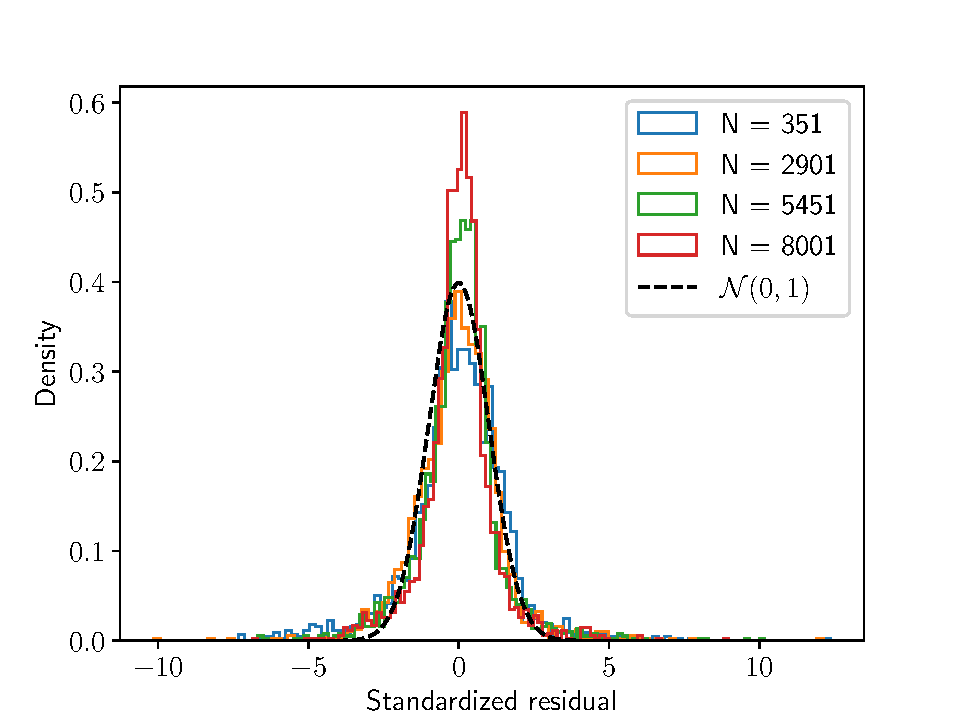
\includegraphics[scale=1]{figures/standardized_residuals/standardized_residual_simple_models.pdf}
    \caption{The figure shows histograms of the standardized residuals computed for 
        different BNNs. The normal distribution is drawn as dotted line. 
    }
    \label{fig:standardized_residual}
\end{figure}
